\documentclass[12pt,oneside,a4paper,english]{article}
\usepackage[T1]{fontenc}
\usepackage[latin2]{inputenc}
\usepackage[margin=2.25cm,headheight=26pt,includeheadfoot]{geometry}
\usepackage[english]{babel}
\usepackage{listings}
\usepackage{color}
\usepackage{titlesec}
\usepackage{titling}
\usepackage[framed, numbered]{matlab-prettifier}
\usepackage{changepage}
\usepackage{amsmath}
\usepackage{hyperref}
\usepackage{enumitem}
\usepackage{graphicx}
\usepackage{fancyhdr}
\usepackage{lastpage}
\usepackage{caption}
\usepackage{tocloft}
\usepackage{setspace}
\usepackage{multirow}
\usepackage{titling}
\usepackage{float}
\usepackage{comment}
\usepackage{booktabs}
\usepackage{indentfirst}
\usepackage{lscape}
\usepackage{booktabs,caption}
\usepackage[flushleft]{threeparttable}
\usepackage[english]{nomencl}
\usepackage{xcolor}
\usepackage{lipsum}


% --- set footer and header ---
\pagestyle{fancy}
\fancyhf{}

\setlength{\parindent}{2em}
\title{Introduction to Aldebaran Characteristics and Spectrum} % to reference as \title, dont use \maketitle
\makeatletter\let\Title\@title\makeatother



\lstset{language=Matlab,
style=Matlab-editor,
basicstyle=\normalsize\mlttfamily,
numbers=left,
numberstyle={\scriptsize\color{black}},			% size of the numbers
numbersep=0.5cm											
}

\newlist{steps}{enumerate}{1}
\setlist[steps, 1]{leftmargin=1.5cm,label = Step \arabic*:}
\renewcommand{\headrulewidth}{1pt}
\renewcommand{\footrulewidth}{1pt}

%\lhead{\Title}
\rhead{\nouppercase{\rightmark}}
\lhead{\Title}
\setlength\headheight{16pt}
\setlength{\footskip}{50pt}
\lhead{\Title} %rightH title
\cfoot{\thepage}

% --- End of page settings ---
\begin{document}
\pagenumbering{arabic} 

\begin{titlepage}
\begin{center}
\vspace{2cm}
%\textsc{ Danmarks Tekniske Universitet}\\[1.5cm]
\vspace{2cm}

\vspace{2cm}

% Title
\hrule
\vspace{.5cm}
{ \huge \bfseries Introduction to Alderbaran Characteristics and Spectrum} % title of the report
\vspace{.5cm}

\hrule
\vspace{1.5cm}

\textsc{\textbf{Authors}}\\
\vspace{.5cm}
\centering

% add your name here
Zachary Shelton 
\vspace{4cm}

\centering \today % Dags dato
\end{center}
\end{titlepage}
\doublespacing
%\addcontentsline{toc}{section}{Table of Contents}
\renewcommand{\baselinestretch}{1}\normalsize
\tableofcontents
\renewcommand{\baselinestretch}{1}\normalsize
%\singlespacing
\thispagestyle{fancy} % force page style
\newpage
\section{Abstract}
There are billions of stars and celestial bodies that are worthwhile for scientist and astronomers to observe. When focusing on one body, it requires navigating various databases and academic journals to find characteristics of the body. This paper will focus on the star Aldebaran, which is the brightest star in the constellation Taurus. The paper will discuss the characteristics of Aldebaran, including its class, lumninosity, and temperature. It will also outline how to find the same information for other celestial bodies. 

\section{Celestial Databases}
There is so much observational data it feels impossible to find a specific piece of data or information. However, there are tools and databases that can help. The first tool is the \href{https://cds.unistra.fr/}{SIMBAD database}, which is a database of astronomical objects. The database provides basic information about celestial bodies, such as their class, mass, and temperature. There is also second tool is the \href{https://vizier.cds.unistra.fr/viz-bin/VizieR}{VizieR database}, which provides detailed information about similar or same celestial bodies, such as their spectral type, luminosity, and radius. If your interested in exoplanets, there is the Exoplanet Archive, which provides information about observed and theorized exoplanets, such as their rotatational velocity radius, and orbital period.

\section{Glossary of Important Terms}
Important Terms and concepts for this tutorial:
\begin{itemize}
    \item \textbf{Stellar Class} - The class of a star is a letter that represents the temperature of the star. The classes are O, B, A, F, G, K, and M. The O class is the hottest and the M class is the coolest, these are described in the Hertzsprung-Russell Diagram. These correspond to the mass and temperature of the star, modern classification include a second classifier that is called the Yerkes Luminosity Classes covering special cases. There is also a 3rd part being a letter grade of how sure the class determination is. \textbf{Sometimes called spectral type.}
\end{itemize}
    \begin{figure}
        \centering
        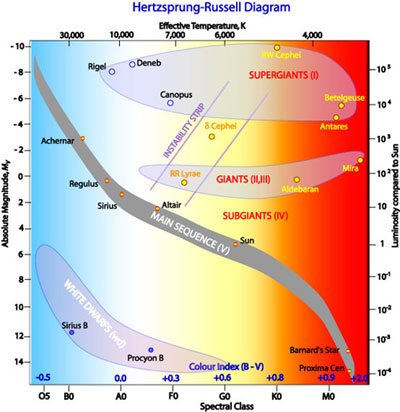
\includegraphics[width=0.54\textwidth]{hrdiagram1.jpg}
        \caption{Hertzsprung-Russell Diagram \cite{hertz}}
        \label{fig:hertz}
    \end{figure}
\begin{itemize}
    \item  \textbf{Blackbody Radiation} - Blackbody radiation is the radiation that is emitted by a blackbody(read more at: \href{https://phys.libretexts.org/Bookshelves/University_Physics/University_Physics_(OpenStax)/University_Physics_III_-_Optics_and_Modern_Physics_(OpenStax)/06%3A_Photons_and_Matter_Waves/6.02%3A_Blackbody_Radiation}{Blackbody Radiation}). Stars release light accross a wide spectrum, light from the same star arrive in different wavelengths, a star could seem dim in the visible spectrum but be very bright in the infared spectrum. The peak wavelength, where most energy is emitted indicates to astronomers what the temperature of the star is.
    \begin{figure}[H]
        \centering
        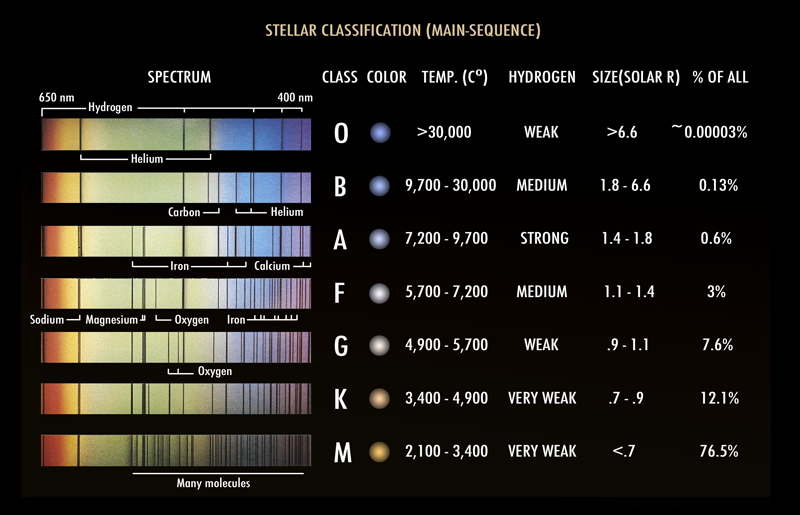
\includegraphics[width=0.9\textwidth]{StellarClassification.png}
        \caption{Stellar Classification Chart \cite{stellerclass}}
        \label{fig:stellarclass}
    \end{figure}
    \item \textbf{Wien's Law} - States the peak wavelength of a blackbody is inversely proportional to the temperature of the blackbody. The law is represented by the equation $\lambda_{\text{max}} = \frac{b}{T}$, where $\lambda_{\text{max}}$ is the peak wavelength, $b=2.89*10^{-3} m \cdot K$ is Wien's constant, and $T$ is the temperature of the blackbody.
    \item \textbf{Stellar Luminosity} - A measure of the total energy a celestial body releases each second, this is also know as absolute brigtness. There are many ways to measure this, and there are definite challenges in determining the true brightness of any stellar body far away.(Read More at: \href{https://www.teachastronomy.com/textbook/Properties-of-Stars/Stellar-Luminosity/}{Stellar Luminosity})
\end{itemize}

\section{Finding Information on Aldebaran}
Heading to \href{https://simbad.cds.unistra.fr/simbad/}{SINBAD}, we can search for Aldebaran and find general characteristics of the star. Aldebaran is an indentifier, however there are many more celestial bodies to give each a unique name, so the identifier is a combination of numbers and letters. The identifier for Aldebaran is HIP 21421 or Alpha Tauri.
\begin{figure}[H]
    \centering
    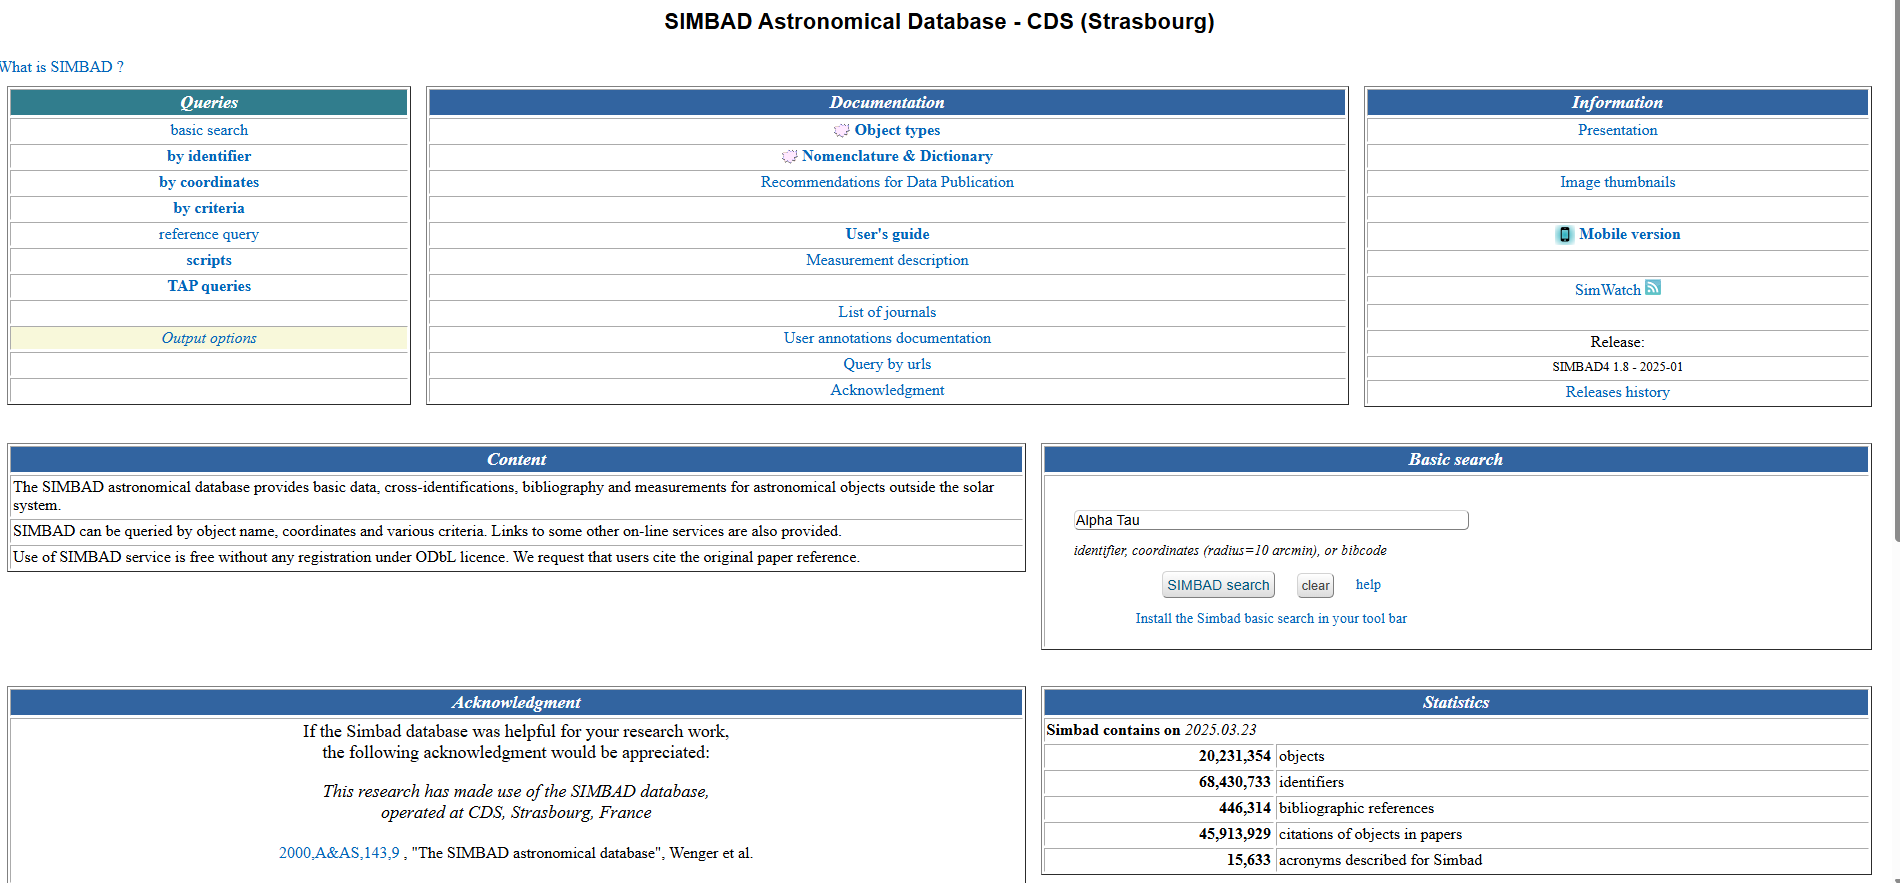
\includegraphics[width=0.9\textwidth]{SINBAD1.png}
    \caption{SIMBAD Database homepage, search for Aldebaran using one of its identifier \cite{simbad}}
\end{figure}
Completing the search will take you directly to the star Aldebaran. The page will show the star's class, lumninosity, and temperature. The class of Aldebaran is K5+III B, which means it is a cool giant star. We will calculate Aldebaran's temperature later using specral data.
\begin{figure}[H]
    \centering
    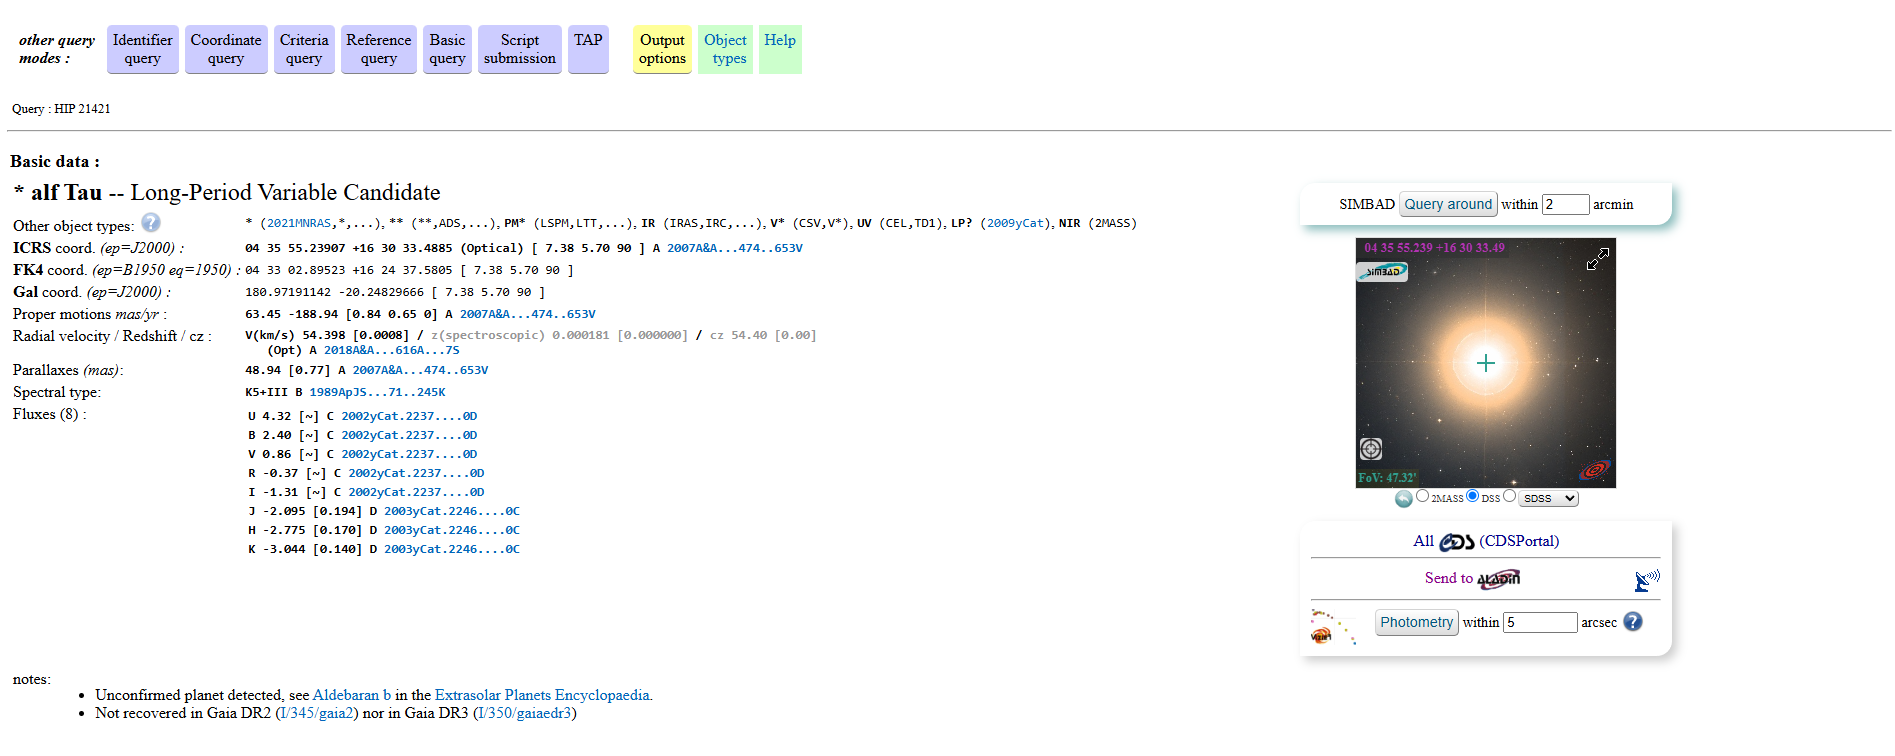
\includegraphics[width=0.9\textwidth]{SINBAD2.png}
    \caption{SIMBAD Database page for Aldebaran, note the class, rotational velocity, and temperature of the star.\cite{simbad}}
\end{figure}
We will include a glossay of terms with their reference in the page, the physical term, and the meaning of the term. 
\begin{table}[H]
    \centering
    \caption{Summary of Terms and the Sections in a SIMBAD Star Page}
    \begin{tabular}{|c|p{3cm}|p{9cm}|}
    \centering
    \textbf{SIMBAD TERM} & \textbf{Physics Term} & \textbf{Definition} \\ \hline \hline
            ICRS coord  & Stellar Coordinates    & Reference location coordinate     \\ \hline   
            FK4 coord   & Stellar Coordinates    & Reference location coordinat(alternate coordinate system).  \\ \hline
            GAL coord   & Stellar Coordinates    & Reference location coordinat(alternate coordinate system).   \\ \hline
            Proper Motions(mas/yr) & Stellar Motion & Motion of star from earth in milliarcseconds per year.  \\ \hline 
            Radial velocity/Redshift/cz & Apparent velocity of star is moving from Earth & Velocity of star from earth in km/s, this is the doppler effect causing redshift.  \\ \hline
            Parallax(mas) & Parallax distance of the star in milliarcseconds & Using this value, the stellar distance to the star can be determined.  \\ \hline
            Spectral type & Stellar Class & The class of the star, refer to above for details. \\ \hline
            Fluxes & Luminosity & Luminosity of the star in various wavelengths starting from U - UV light to K - infared light \\ \hline
            Hierarchy & Objects in the stars orbit or vice versa & Can be planets, other stars, generally organizes with orbiting bodies being children of larger bodies. \\ \hline
            Identifier & Acronym Information & Due to the amount of data, there are many different nomenclature used, so clicking one of thes can give insight.  \\ \hline
            References & Academic Observations & Allows for historical review of past observational data and the read on the methodology used. \\ \hline
            Collections of Measurements & Measurements  & Direct link to measurements made by scientist with a reference to the academic article. See Section 5.  \\ \hline
            Observing logs & Observational Data & Link to raw observational data, this could be unformatted.  \\ \hline
            External Archives & External Databases & Links to other databases that may have more information on the star.  \\ \hline
    \end{tabular}
    \label{tab:table1}
\end{table}
\newpage
\section{Aldebaran's Spectrum and Characteristics}
Scrolling down, we can find Aldebaran's references in academic jourunals and more importantly, measurements and observational data. Looking at \textbf{SpT} measurements will show every measurement of Aldebaran's spectrum and its classification. You can see the classification and the journal that classified it. There are 3 columns, ds/s refers to the method(if known) that was used to collect the data and make the classification which is in column 2. The third column is a link to the academic journal that published the data.
\begin{figure}[H]
    \centering
    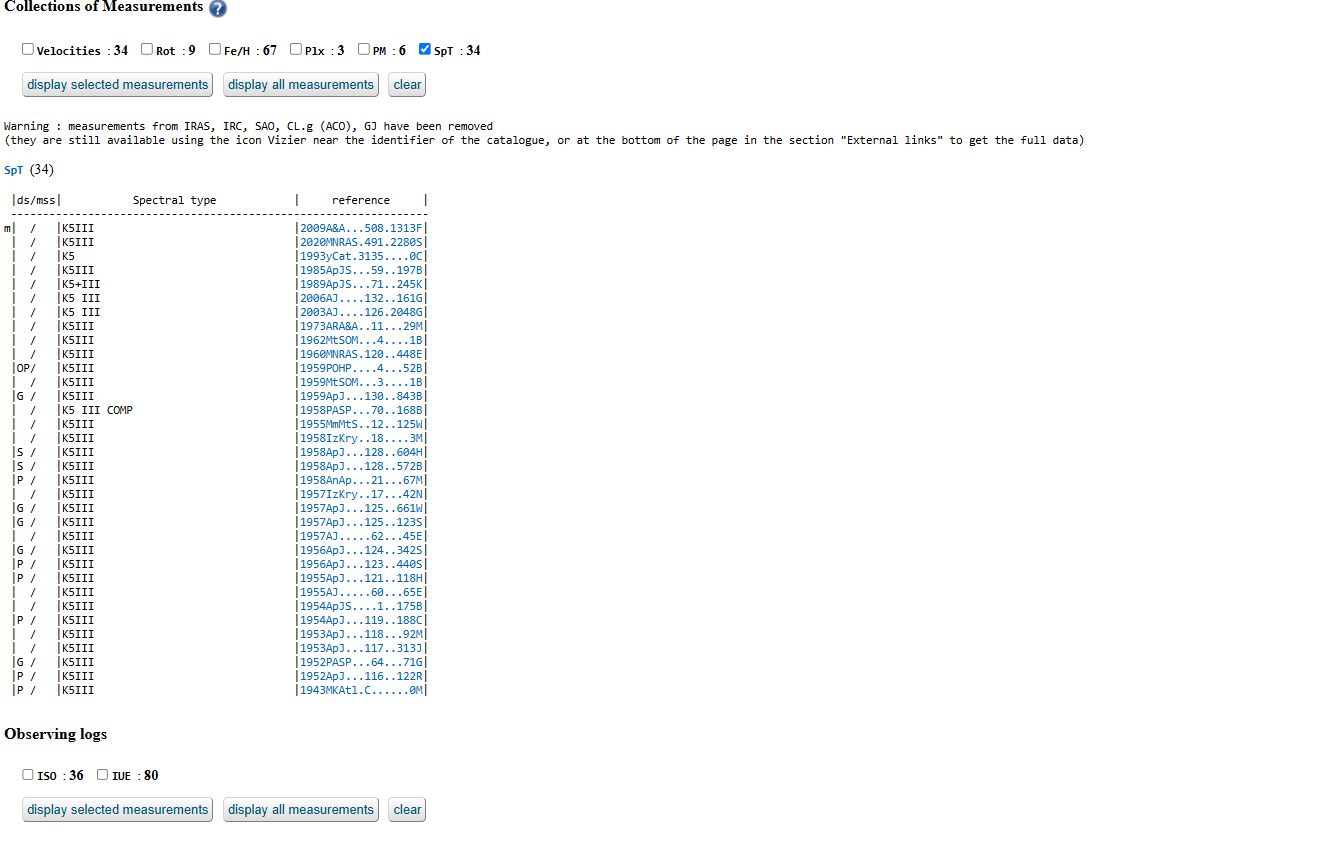
\includegraphics[width=0.9\textwidth]{SINBAD3.png}
    \caption{SIMBAD spectrum measurements and classifications of the Aldebaran.\cite{simbad}}
\end{figure}
If you are beginning a search or want to look for many stars of a certain characteristic or specification, starting with SIMBAD to find them is best as you can search by stellar coordinate or by a characteristic. 
\newpage
\section{VizieR Database}
In order to better visualize the data, you can use the VizieR database to find more detailed information about the star. We can head directly from the SIMBAD page to the VizieR page by clicking photometry button, which will take you to the VizieR page for the region of the sky that Aldebaran is in.
\begin{figure}[H]
    \centering
    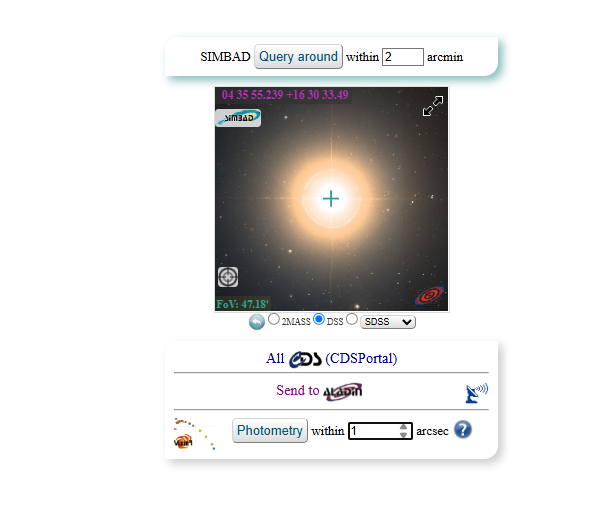
\includegraphics[width=0.9\textwidth]{SINBAD4.png}
    \caption{Photometry link used in SIMBAD leading the VizieR database. Note: that the arcsec is set to 1.\cite{sinbad}}
    \label{fig:sinbadphotometry}
\end{figure}
We are led to VizieR's database showing observational data of the region of the sky that Aldebaran is in. The data is organized by the type of data and the journal that published the data.
\begin{figure}[H]
    \centering
    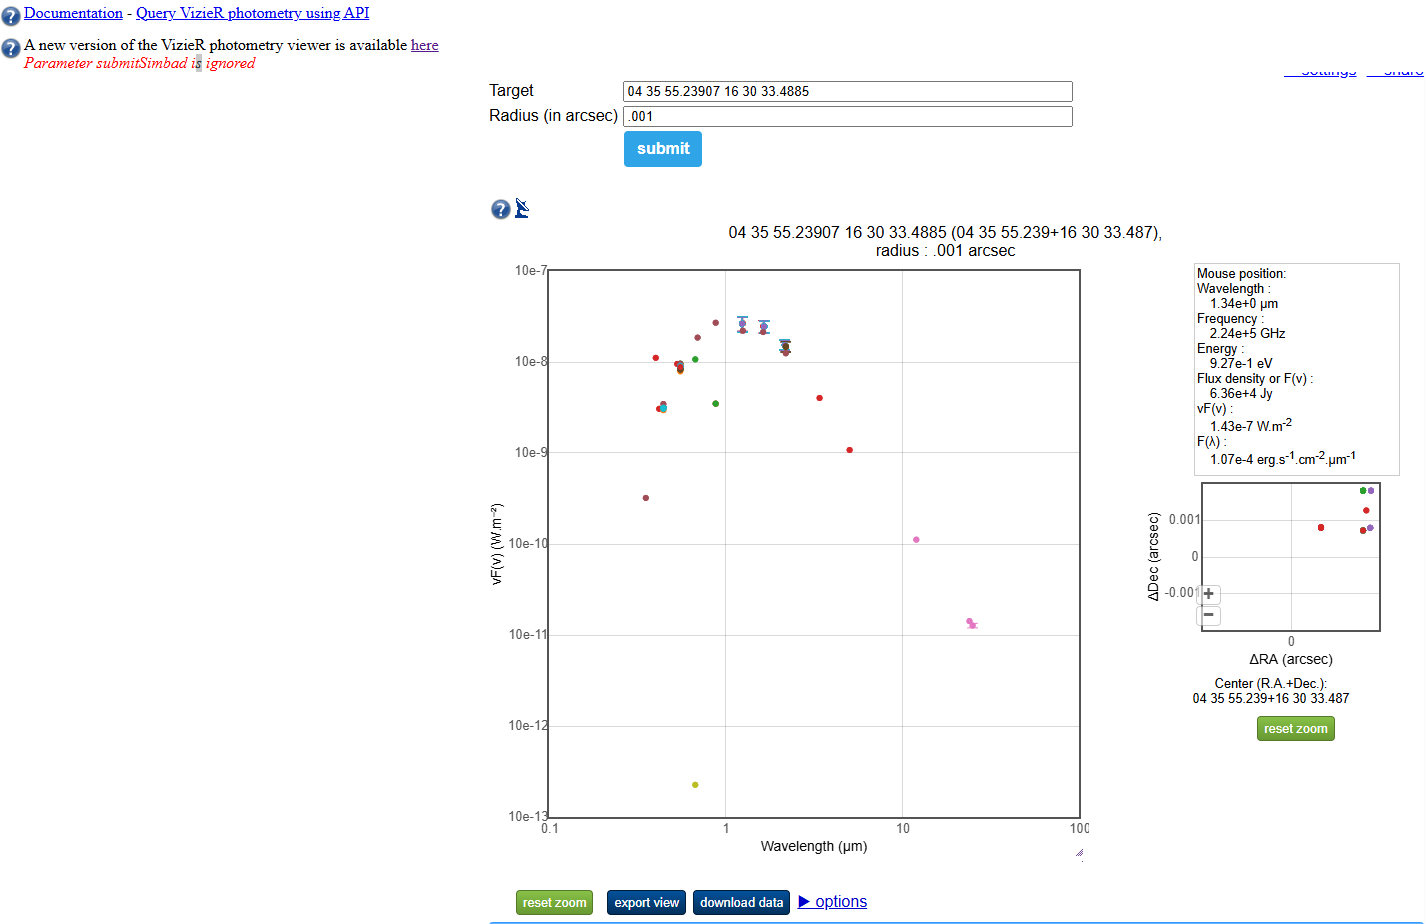
\includegraphics[width=0.9\textwidth]{VizieR1.png}
    \caption{VizieR database page for the region of the sky that Aldebaran is in\cite{vizier}}
    \label{fig:vizier}
\end{figure}
There are 2 plots, the first(left) plot is the spectral energy distribution of the star, which shows the energy output(or flux) of the star at different wavelengths. The second smaller(right) plot of stellar coordinates of the measurements, there are many measurements in the same location at different spectra in order to get a clear idea of the what the star's temperature is. Scrolling down will show the data in a table format. In order to export these values, you must utilize VizieR's API or download the data to read with VizieR's software.

Lets look at the left plot more closely in figure: \ref{fig:vizier2}, the y-axis corresponds to the flux in watts per square meter($W \cdot m^{-2}$), this value is a measure of the absolute luminosity, absolute means determine in the frame of the star, what the stars actual energy output(brightness) and is not what we see on earth, this is determined via using parallax to determine the red shift of incoming light. The x a-xis corresponds to the wavelength of the light in micrometers, this plots y-axis is logarithmic to help determine the peak emission wavelength.
\begin{figure}[H]
    \centering
    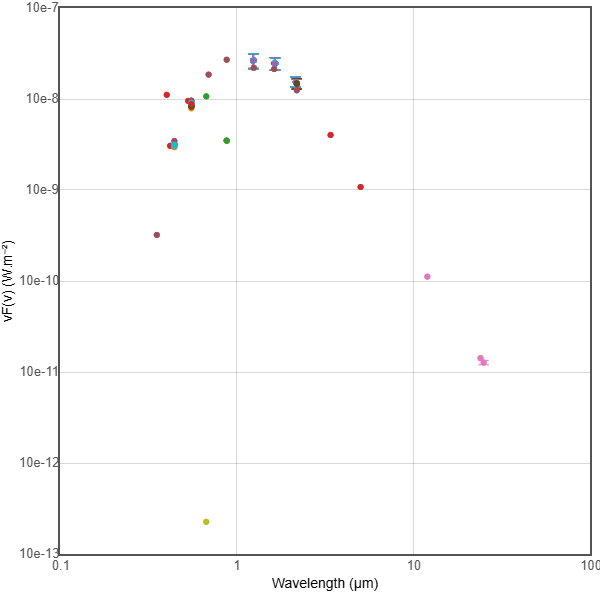
\includegraphics[width=0.9\textwidth]{VizieR2.png}
    \caption{Spectrum Plot of Aldebaran in \cite{vizier}}
    \label{fig:vizier2}
\end{figure}
\section{Determining the Temperature of Aldebaran}
Based on the plot of \ref{fig:vizier2}, the peak flux emitted is at the wavelength 878 $\mu m$ or 878 $nm$, this wavelength in the infared spectrum. Implement Wien's Law:
$$
\lambda_{\text{max}} = 8.78*10^{-7} = \frac{2.89*10^{-3}}{T}
$$
Leading to:
$$
T = \frac{1}{.000303} \approx 3291 K
$$
This is based on the peak wavelength emitted by Aldebaran, Wien's Law states that the peak wavelength and the temperature are inversely proportional.

\section{Spectrum Analysis of Stars and Aldebaran}
Spectrum analysis is inherently difficult for many reasons, the first is dealing with light absorbtion by our atmosphere. If the telescope is on earth, incoming light is absorbed or refracted by our atmosphere, this problem is solved in general by spaceborne telescopes and placing them high in the atmosphere. Fortunately, most measurements account for this and are included in as an error.(seen in \ref{fig:vizier} as bars above a point) Next, is accounting for redshifting due to the doppler effect. In Aldebaran's case, the star is fortunately close enough that observers can accurately measure the redshifting of light from it, in this tutorial how redshift is determined specifically will be glossed over for 3 reasons: 
\begin{itemize}
    \item It is not effective for all stars at longer distance >3200 lightyear
    \item There are many phenomena that are doppler effects like gravitational lensing
    \item Its uncertain that the redshift is locally(ie near the star) the same consistently.
\end{itemize}
It's complicated and while learning astronomy and astorphysics, we can assume that scientist are doing their best to account for these errors. With a finer analysis of the spectrum we can idenify lines in the spectra, these correspond to an element present in the atmosphere of the sun absorbing outgoing light, these studies are intensive and not always done in space surveys, where most citizen scientist find observational data. These are general photos taken over a portion of the night sky looking in a single band of light. In 2016, Eyal Schwartz and others were able to identify spectral lines in Aldebaran in a study to improve methods of identifying exoplanets, Aldebaran is believed to have an exoplanet named Aldebaran b. This study was intensive involving many repeated observations at many different wavelengths. The paper shows that the Aldebaran is burning metal like sodium and magnesium \cite{schwartz}, this is generally in line with red giants(K-band stars). We can assume that the star is a metal rich star in its later stages of life based on the hertzsprung-russell diagram. 

\newpage
\section{Conclusion and Extensions}
In conclusion, Aldebaran is a cool class K star with a temperature of 3291 K. The star is a metal rich star in its later stages of life. The same study can be applied to any star, as we begin to unravel more accurate methods to simulate celestial bodies and spectra, we can identify things like exoplanets transiting in front of stars and more accurate pictures of the matter composition of stars. Utilizing NASA Exoplanet survey, GAIA archives along with VizieR and SIMBAD, you can find more info on any known phenomena in the night sky.

\addcontentsline{toc}{section}{References}
\bibliography{document.bib} 
\bibliographystyle{ieeetr}

\label{endOfDoc}
\end{document}